\chapter*{Wprowadzenie}
\addcontentsline{toc}{chapter}{Wprowadzenie}
\label{cha:wstep}

AVR to rodzina mikroprocesorów opracowana i~rozwijana przez firmę Atmel. Oparta o~nią jest między innymi platforma Arduino, która~-- jak~przedstawiono na~rysunku \ref{fig:arduinotrends} -- z~roku na~rok zyskuje popularność. Platforma Arduino zaprojektowana została z~myślą o~projektach tworzonych nie tylko przez inżynierów, lecz także artystów i~projektantów~\cite{BanShi14}. Jest ona też często używana do~prototypowania urządzeń wpisujących się w~koncepcję Internetu Rzeczy \emph{(ang. Internet of Things, IoT)}.

\begin{figure}[h]
\centering
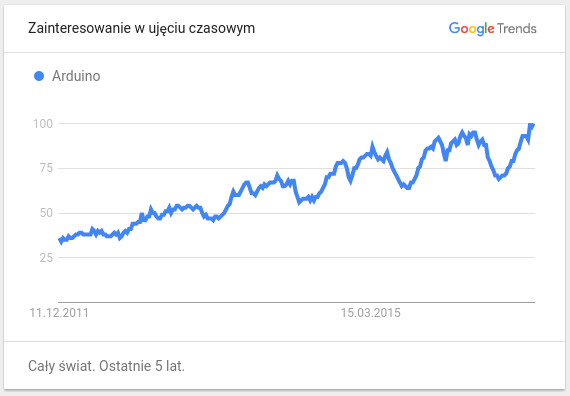
\includegraphics[width=0.7\textwidth]{images/arduino-trends.png}
\caption{Relatywna liczba wyszukiwań frazy ,,Arduino'' w ostatnich pięciu latach. Źródło: Google Trends}
\label{fig:arduinotrends}
\end{figure}

Urządzenia wbudowane podłączone do~Internetu są szczególnie narażone na~ataki. W~2016 roku podatne urządzenia wbudowane zostały wykorzystane do~przeprowadzenia masywnych ataków typu DDoS~\cite{AkaIOT}. Zagrożone są też rozwiązania oparte o~komunikację bezprzewodową jak~Wi-Fi oraz~Bluetooth. Istotne jest więc dostarczenie narzędzi, które~pozwalają nie tylko na~szybkie prototypowanie, ale~także na~zachowanie bezpieczeństwa takich rozwiązań jak~bezprzewodowe tokeny, czujniki, sprzętowe menadżery haseł czy~inteligentne domy.

W~niniejszej pracy przedstawiono protokół bezpiecznej komunikacji oraz~bibliotekę programistyczną zaprojektowane z~myślą o~prostocie integracji. Wybrane zostały zestawy algorytmów, które~zapewniają bezpieczeństwo komunikacji. Ich złożoność została ukryta za~interfejsem programistycznym, który~ogranicza możliwość wprowadzenia błędów zmniejszających bezpieczeństwo. Zaproponowane rozwiązanie zapewnia poufność, autentyczność oraz~integralność przesyłanych danych.

W~rozdziale \ref{cha:metodyUwierzytelniania} przedstawione zostały różne metody uwierzytelniania i~uzasadniony został wybór konkretnych algorytmów. Implementacja została szczegółowo opisana w~rozdziale \ref{cha:implementacja}. Całość została zweryfikowana poprzez~strzorzenie przykładowego oprogramowania oraz~porównanie z~implementacją na~inną platformę, co opisano w~rozdziale \ref{cha:walidacja}. W~podsumowaniu przedstawiono całe rozwiązanie oraz~jego ograniczenia i~słabe strony.

Całość kodu źródłowego dostępna jest na~licencji MIT w~serwisie GitHub\footnote{\url{https://github.com/kacperzuk/seconn}}.
